%! Author = joels
%! Date = 24/12/2020

\section{Standard Container \& Iterators}
% You know the properties of the different standard containers
% You can select the best standard containers for your application
% You know the different iterator categories and their capabilities
% You can explain the difference between a const iterator and a const_iterator

\subsection{STL Containers: General API}
\begin{itemize}
    \item Sequence Containers
        \SubItem{Elements are accessible in order as they were inserted created}
        \SubItem{Find in linear time through the algorithm find}
    \item Associative Containers
        \SubItem{Elements are accessible in sorted order}
        \SubItem{find as member function in logarithmic time}
    \item Hashed Containers
        \SubItem{Elements are accessible in unspecified order}
        \SubItem{find as member function in constant time}
\end{itemize}
\begin{center}
    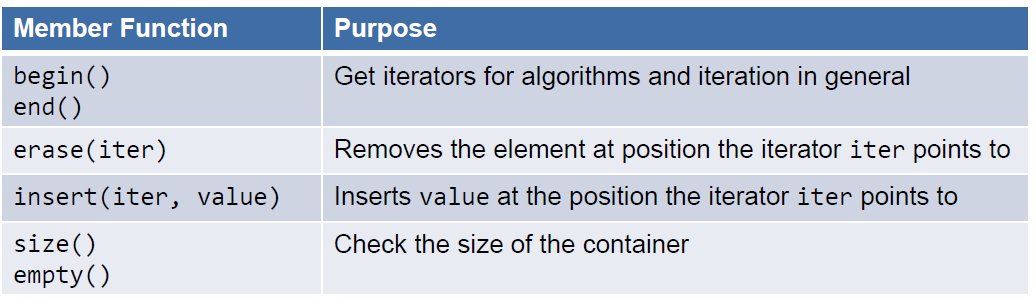
\includegraphics[scale=0.45]{container_functions.png}
\end{center}

\subsection{Sequence Containers}
\subsubsection{std::vector \& std::array}
Siehe Kapitel3: Sequences and Iterators (Seite 6)
\subsubsection{std::deque$<$T$>$ $\rightarrow$ \#include$<$deque$>$}
std::deque is like std::vector but with additional, efficient front insertion/removal
\begin{center}
    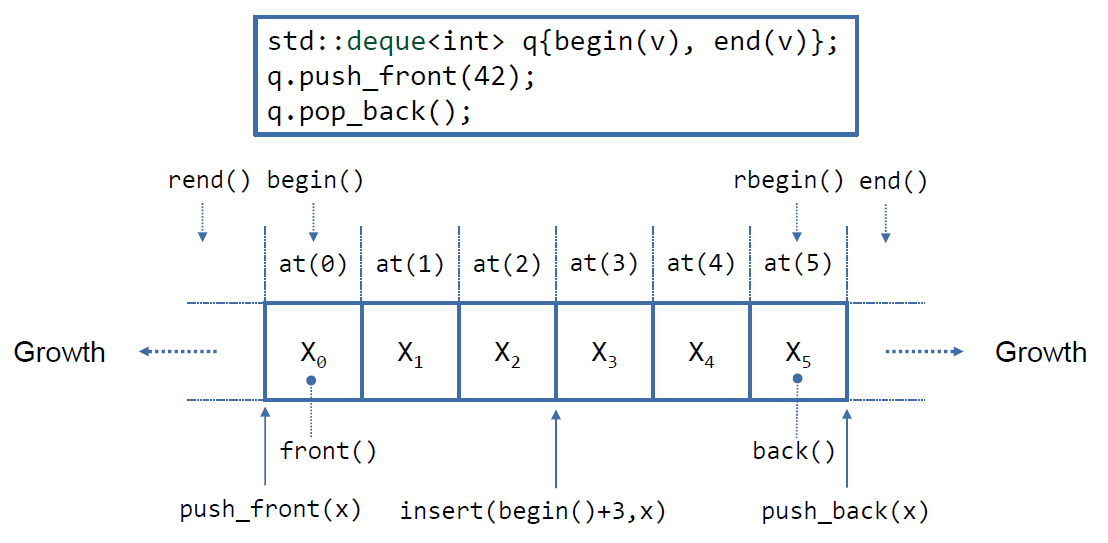
\includegraphics[scale=0.43]{deque.png}
\end{center}
\subsubsection{std::list$<$T$>$ $\rightarrow$ \#include$<$list$>$}
Efficient insertion in any position. Lower efficiency in bulk operations. Requires member function call for sort etc. Only bi directional iterators no index access
\begin{center}
    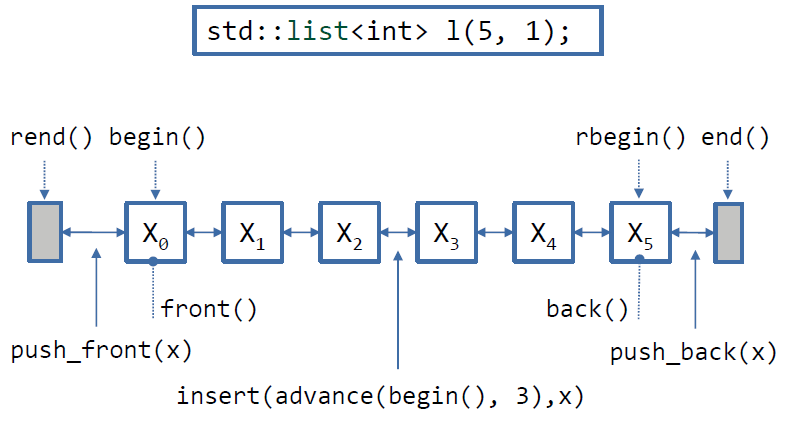
\includegraphics[scale=0.43]{list.png}
\end{center}
\subsubsection{std::forward\_list$<$T$>$ $\rightarrow$ \#include$<$forward\_list$>$}
Efficient insertion AFTER any position, but clumsy with iterator to get \dq before\dq position. Only forward iterators, clumsy to search and remove, use member functions not algorithms.
\begin{center}
    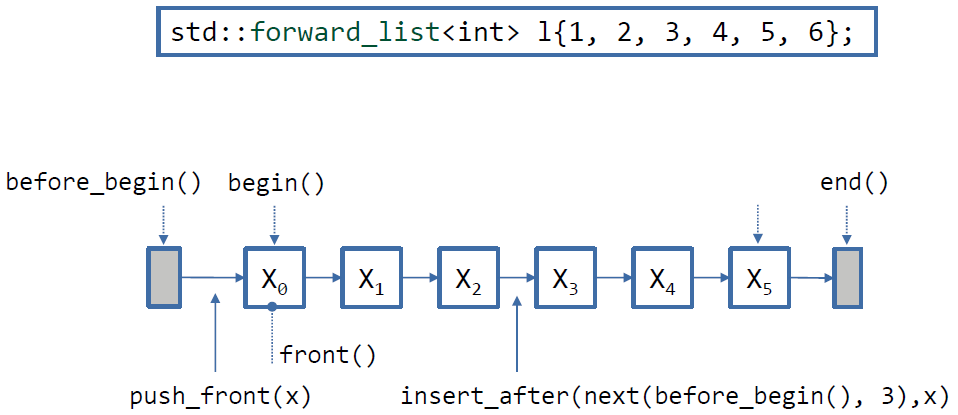
\includegraphics[scale=0.45]{forward_list}
\end{center}
\subsubsection{std::stack $\rightarrow$ \#include$<$stack$>$}
Uses std::deque (or std::vector, std::list) and limits its functionality to stack operations. Iteration not possible.
\begin{center}
    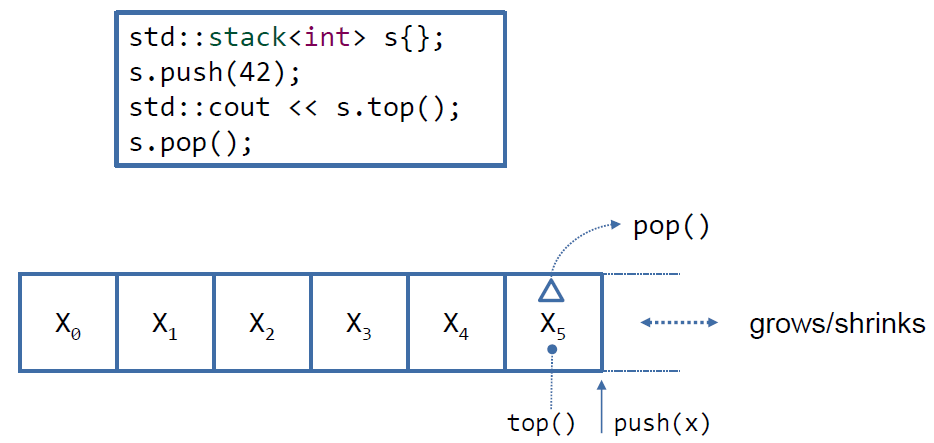
\includegraphics[scale=0.45]{stack.png}
\end{center}
\subsubsection{std::queue $\rightarrow$ \#include$<$queue$>$}
Uses std::deque (or std::list) and limits its functionality to queue operations. Iteration not possible.
\begin{center}
    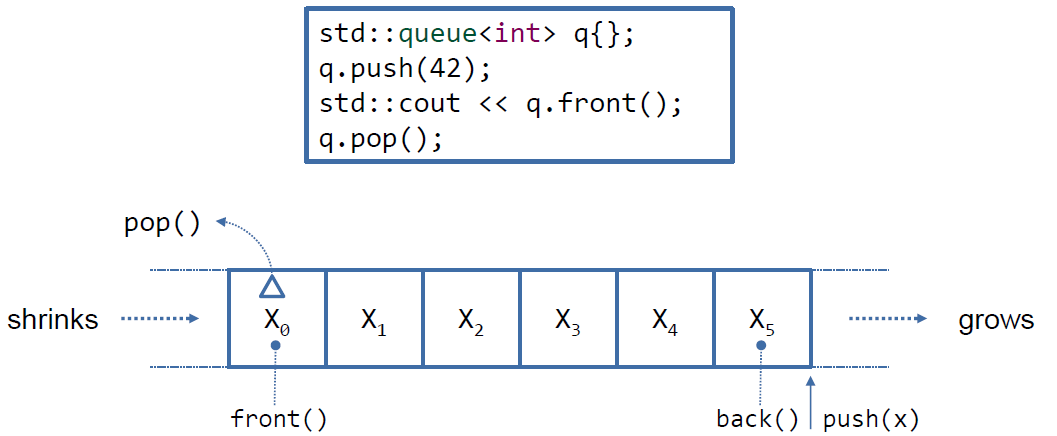
\includegraphics[scale=0.45]{queue.png}
\end{center}
\subsubsection{std::priority\_queue $\rightarrow$ \#include$<$stack$>$}
Uses std::deque (or std::vector) and limits its functionality to stack operations. top() element is always the smallest.
\begin{center}
    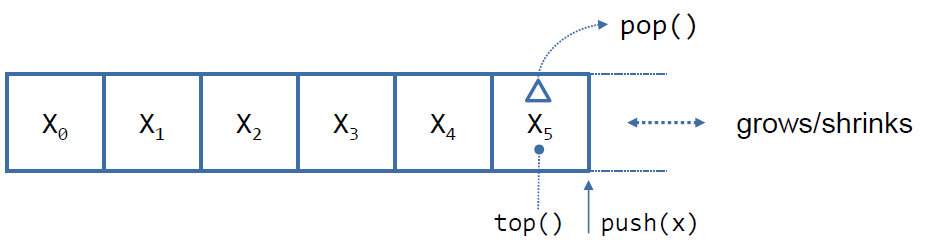
\includegraphics[scale=0.45]{priority_queue.png}
\end{center}
\subsection{Associative Containers}
\begin{center}
    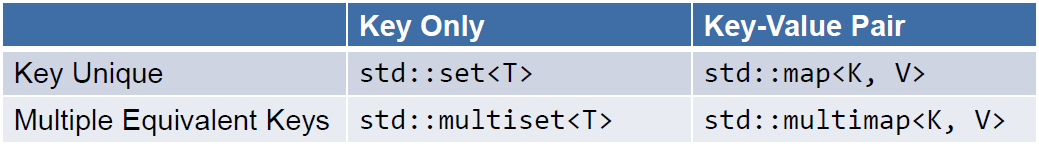
\includegraphics[scale=0.45]{associative_containers.png}
\end{center}
\subsubsection{std::set $\rightarrow$ \#include $<$set$>$}
\begin{itemize}
    \item std::set$<$int$>$ values$\{$7, 1, 4, 3, 2, 5, 6$\}$
    \item Stores elements in sorted order (ascending by default)
    \item Iteration walks over the elements in order
    \item Member functions to check if element exists: .find(element) or .count(element)
\end{itemize}
\subsubsection{std::map $\rightarrow$ \#include $<$map$>$}
Stores key-value pairs in sorted order. Default: By key ascending.\\
Use .first() for key and .second() for value.
\begin{center}
    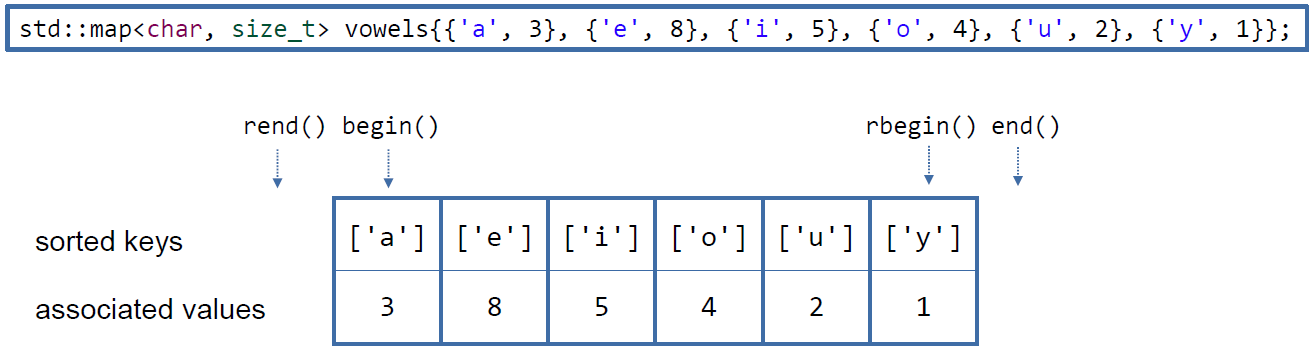
\includegraphics[scale=0.45]{map.png}
\end{center}
\subsubsection{std::multiset $\rightarrow$ \#include $<$set$>$, std::multimap $\rightarrow $\#include $<$map$>$}
Multiple equivalent keys allowed. Use equal\_range() or lower\_bound()/upper\_bound() member functions to find boundaries of equivalent keys.
\begin{center}
    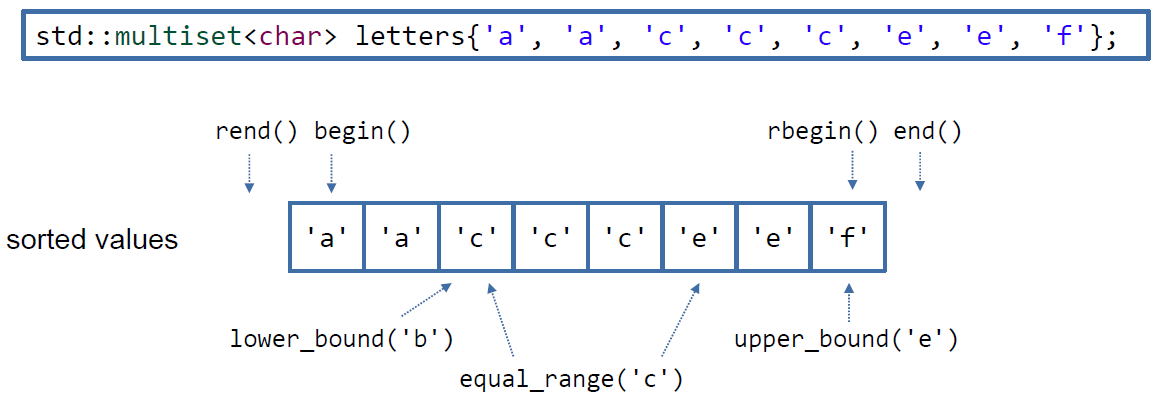
\includegraphics[scale=0.45]{multiset.png}
\end{center}
\subsection{Hashed Containers}
\subsubsection{std::unordered\_set $\rightarrow$ \#include $<$unordered\_set$>$, std::unordered\_map $\rightarrow$ \#include $<$unordered\_map$>$}
Usage is almost equivalent to std::set/std::map. Except for the lack of ordering.

\subsection{Iterators}
What are these Iterator Categories for?
\begin{itemize}
    \item Some algorithms only work with powerful iterators, e.g: std::sort() requires a pair of random access iterators (it needs to jump forward and backward)
    \item Some algorithms can be implemented better with more powerful iterators, e.g: std::advance() or std::distance()
\end{itemize}
\subsubsection{Input Iterator}
\begin{itemize}
    \item Supports reading the current element (of type Element)
    \item Allows for one-pass input algorithms (cannot step backwards)
    \item Models the \textcolor{blue}{std::istream\_iterator} and \textcolor{blue}{std::istream}
    \item Can be compared with == and != to other iterator objects of the same type: \textcolor{blue}{It}
    \item Can be copied (after increment all other copies are invalid!)
\end{itemize}
\subsubsection{Forward Iterator}
\begin{itemize}
    \item Can do whatever an input iterator can, plus: Supports changing the current element
    \item Allows only for one-pass input algorithms
    \item Models the \textcolor{blue}{std::forward\_list} iterators
\end{itemize}
\subsubsection{Bidirectional Iterator}
\begin{itemize}
    \item Can do whatever a forward iterator can, plus: Can go backwards
    \item Allows for forward-backward-pass algorithms
    \item Models the \textcolor{blue}{std::set} iterators
\end{itemize}
\subsubsection{Random Access Iterator}
\begin{itemize}
    \item Can do whatever a bidrectional iterator can, plus:
        \SubItem{Directly access element at index}
        \SubItem{Go n steps forward or backward}
        \SubItem{Subtact two iterators to get the distance}
        \SubItem{Compare with relational operators ($<$, $<$=, $>$, $>$=)}
    \item Allows random access in algorithms
    \item Models the \textcolor{blue}{std::vector} iterators
\end{itemize}
\subsubsection{Output Iterator}
\begin{itemize}
    \item Can write value to current element, but only once
    \item Modeled after \textcolor{blue}{std::ostream\_iterator}
\end{itemize}
\subsubsection{Iterator Functions $\rightarrow$ \#include $<$iterator$>$}
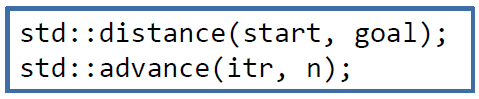
\includegraphics[scale=0.45]{iterator_functions.png}
\begin{itemize}
    \item std::distance() counts the number of hops iterator start must make until it reaches goal
    \item std::advance() lets itr hop n times
\end{itemize}
\subsubsection{std::advance vs. std::next}
\begin{lstlisting}[style=frame, style= linenumbers, language=C]
int main() {
    std::vector<int> primes{2, 3, 5, 7, 11, 13};

    auto current = std::begin(primes);
    auto afterNext = std::next(current);
    std::cout << "current: " << *current << " afterNext: " << *afterNext << '\n';

    std::advance(current, 1);
    std::cout << "current: "<< *current << " afterNext: " << *afterNext << '\n';
}
\end{lstlisting}